
\section{Katsetus Windowsi peal}\label{sec:katsetus}
Esimese sammuna kella töö analüüsimises prooviti jooksutada Polari enda olemasolevat programmi Windowsi platvormil.
Rakenduse käivitamisel töötas ka Wireshark, millega vaadeldi USB liinidel toimuvat liiklust.
Rakendusse logiti sisse ning pandi see andmeid sünkroonima.
Hetkest, mil rakendus pandi andmeid sünkroonima, edastati 10 paketti.

\begin{figure}[ht]
    \centering
    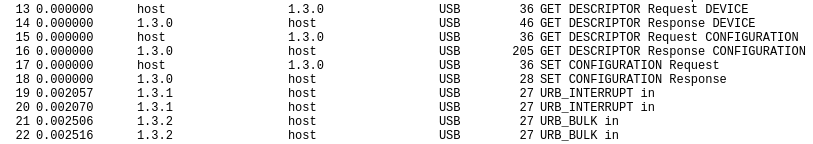
\includegraphics[width=.9\textwidth]{figures/wireshark_packets.png}
    \caption{\textit{Pilt kella ja arvuti vahel liikunud pakettidest}}
    \label{fig:packets}
\end{figure}

Kui need 10 paketti jooniselt~\ref{fig:packets} edastatud olid, katkestas programm töö.
Kasutajale edastati teade, et seadet ei toetata ja polarpersonaltrainer.com ei tööta enam, kuid seadet saab kasutada eraldiseisvana, andmeid sealt enam vaadata arvutis ei saa.

Edasine töö kujutas endast saadud tulemuste proovitud emuleerimist.

\section{Arenduskäik}\label{sec:arendus}
Programmi arendati iteratsioonidega.
Kokku läbiti 2 iteratsiooni, mida järgnevalt kirjeldatakse.

\subsection{Esimene iteratsioon}
Programmi koodi kirjutamist alustati libusb teegiga tutvumisest.
Leiti juhend ning tutvuti selle sisuga ning loeti ka dokumentatsiooni.
Esimese iteratsiooni lõpuks oli olemas koodijupp, mis suutis leida arvuti külge ühendatud seadmete hulgast õige seadme, mida vajas ja suutis selle enda külge saada.

Esimene iteratsioon oli kõige ajamahukam, kuna eelenvalt poldud kursis kella ja teegi tööpõhimõttega. 
Kõige keerulisem oli aru saada sellest, kuidas üldse USB seadmetega suhtlus toimima peaks rakenduses ja mis operatsioone millises järjestuses täpsemalt tegema peaks.

\subsection{Teine iteratsioon}
Teine iteratsioon läks kergemalt ja kiiremini, kuna leiti sarnane projekt.
Leitud projekt oli flowlink\cite{flowlink-git} githubis.
Enda rakenduse koodi ja leitud projekti andmete hankimise osa prooviti ühendada, kuna flowlink oli ühel mudelil toimiv ja testitud ning seega vähendas eksimisvõimalusi enda programmi kirjutamisel.

Selles iteratsioonis kulus suur osa ajast leitud projekti uurimisele ja selle käima panemine enda masinal.
Prooviti ka projekti fookuses olnud kella sellega kasutada, kuid edutult.
Seda projekti uurides selgus, et erinevad mudelid Polari kelladest kasutavad erinevaid käsklusi andmete kättesaamiseks, mis raskendab oluliselt rakenduse loomist.

Iteratsiooni tulemusena kasutusel olev kood lühenes ja liigendus rohkem, kuna esimesel korral kirjutati kogu programmiloogika rangelt 1 faili, kust mõned abifunktsioonid liigutati eralgi \textit{header} faili.